\documentclass[11pt]{article}
\usepackage[margin=1in]{geometry}
\usepackage{amsmath, amssymb, amsthm}
\usepackage{tikz}
\usepackage{pgfplots}
\pgfplotsset{compat=1.17}
\usetikzlibrary{arrows.meta, angles, quotes, decorations.markings, calc}
\usepackage{tcolorbox}
\tcbuselibrary{skins,breakable}
\usepackage{fancyhdr}
\usepackage[hidelinks]{hyperref}
\usepackage{parskip}
\usepackage{multicol}

\newtcolorbox{aside}[1]{colback=yellow!7!white, colframe=yellow!55!black, fonttitle=\bfseries, title=#1, breakable, enhanced}

\pagestyle{fancy}
\fancyhf{}
\rhead{fizicyst}
\lhead{Celestial Mechanics}
\rfoot{\thepage}

\begin{document}

\begin{titlepage}
\begin{center}
{\Huge \textbf{Celestial Mechanics}}\\\vspace{0.5cm}
{\Large Vaibhav Chandra}
\end{center}

\vspace{0.8cm}
\hrule

\vspace{0.4cm}
\begin{multicols}{2}
  \tableofcontents
\end{multicols}

\vspace{0.4cm}
\hrule

\vspace{0.8cm}
\noindent\textbf{Prerequisite Knowledge}
\begin{itemize}
  \item Newton's laws of motion, and basic circular motion (centripetal force)
  \item Vectors: dot and cross products, and their geometric meaning
  \item Basic differentiation and integration (power rule, chain rule)
  \item Comfort with polar coordinates is helpful, but is built up from scratch here
\end{itemize}

\end{titlepage}

\section{Newton's Laws of Gravitation}

Let's start with something almost embarrassingly simple, and then notice why it's actually one of
the most astonishing statements ever made about nature.

Newton's claim was this: \emph{every} pair of masses in the universe pulls on each other. Not just
the Earth and the Moon, not just planets and the Sun --- literally you and the chair you're
sitting in are gravitationally attracted to each other right now. The force is tiny, of course,
because gravity is an extraordinarily weak force compared to, say, the electric force between two
charges. But it's there, and Newton wrote down exactly how strong it is:
\[
\vec F = -\frac{GMm}{r^2}\,\hat r.
\]

Read this slowly. $M$ and $m$ are the two masses. $r$ is the distance between their centers. And
$G$ is a tiny number, $6.674\times10^{-11}\ \mathrm{N\,m^2\,kg^{-2}}$, whose smallness is precisely
why you don't feel yourself being pulled toward your chair --- the masses involved (a person, a
chair) are just too small for this feeble force to be noticeable. It takes something the size of a
\emph{planet} to make gravity impressive.

The minus sign and the $\hat r$ (a unit vector pointing from $M$ toward $m$) are just bookkeeping
to say: the force always points \emph{back} toward the other mass. Gravity never pushes, it only
pulls. This is worth sitting with for a second, because it's not obvious a priori that nature had
to work this way --- electric charges, after all, can either attract or repel depending on their
sign. Mass has no such sign. There's no such thing as "negative mass" that would make gravity
repulsive. Every mass, no exceptions, only attracts.

Now here's the part that made Newton's law so revolutionary at the time: the very same $1/r^2$ law
that makes an apple fall from a tree also keeps the Moon in orbit around the Earth, and the Earth
in orbit around the Sun. Before Newton, people genuinely believed that "the heavens" ran on
completely different rules than "the Earth" did --- that celestial motion was some perfect,
eternal, circular clockwork, fundamentally unlike the messy business of things falling down here
on the ground. Newton's insight was that there is no difference. The Moon is falling, all the
time, exactly the way an apple falls --- it's just moving sideways fast enough that as it falls,
the ground (in this case, the curved surface implied by the Earth's gravity) keeps "falling away"
underneath it at the same rate. That's what an orbit \emph{is}: a continuous fall that never quite
lands.

\subsection*{Gravitational Fields}

It's often convenient to stop thinking about the force on a \emph{specific} mass $m$, and instead
ask: what would the force be on \emph{any} mass placed at this point in space? Dividing the force
by the test mass $m$ gives us the gravitational field,
\[
\vec g(\vec r) = \frac{\vec F}{m} = -\frac{GM}{r^2}\hat r,
\]
which depends only on the source $M$ and the location, not on whatever test mass we imagine
placing there. Think of it like a landscape of "pull" that exists in space whether or not
anything is there to feel it --- much like how a river has a current everywhere, whether or not
there's a boat on it to be swept along.

One beautiful and enormously useful fact about gravitational fields: they add up. If you have
several masses scattered around, the total field at any point is just the vector sum of what each
mass would contribute on its own, as if the others weren't even there. This is called the
\textbf{principle of superposition}, and it's what lets us compute the field of complicated shapes
--- spheres, rings, disks, even lumpy asteroids --- by imagining them chopped into a huge number of
tiny point masses and adding up all their individual pulls.

\subsection*{A Word on "Central" Forces}

Notice something about gravity's structure: its strength depends \emph{only} on the distance $r$,
and its direction is \emph{always} along the line connecting the two masses. A force like this ---
depends only on distance, always points along the radius --- is called a \textbf{central force}.
It sounds like a small, technical observation. It is anything but. As we're about to see, this one
property, all by itself, is responsible for essentially everything Kepler discovered about
planetary motion, centuries before anyone knew \emph{why} his laws were true. Kepler found the
rules by painstakingly staring at Tycho Brahe's observational data; we're going to derive the same
rules by staring at one simple structural fact about the force itself.

\section{Kepler's Laws for Circular and Non-Circular Orbits}

\subsection{Why Being ``Central'' is Such a Big Deal}

Here's a question worth pausing on: why does a planet's orbit stay in a flat plane at all? Why
doesn't the Earth, say, gradually wander up and down out of the plane it orbits in, tracing some
complicated three-dimensional squiggle around the Sun?

The answer comes from a quantity called \textbf{angular momentum}, defined as
\[
\vec L = m(\vec r\times\vec v).
\]
If you haven't spent time with cross products, here's the idea: $\vec r\times\vec v$ produces a new
vector that is perpendicular to \emph{both} $\vec r$ and $\vec v$ --- think of it like the axle of a
spinning wheel, pointing straight out of the plane that the wheel spins in, at a right angle to
everything happening in that plane.

Now let's ask how $\vec L$ changes with time:
\[
\frac{d\vec L}{dt} = m\left(\frac{d\vec r}{dt}\times\vec v\right) + m\left(\vec r\times\frac{d\vec v}{dt}\right)
= m(\vec v\times\vec v) + \vec r\times(m\vec a) = \vec r\times\vec F.
\]
The first term vanished because any vector crossed with itself is always zero (there's no "twist"
between a vector and its own direction). We're left with $\vec r\times\vec F$. And here's where
centrality earns its keep: since the gravitational force $\vec F=F(r)\hat r$ points \emph{along}
$\vec r$, the two vectors are parallel, and the cross product of parallel vectors is zero. So:
\[
\boxed{\frac{d\vec L}{dt} = 0.}
\]
Angular momentum doesn't change. Not its size, not its direction. Ever. For as long as the force
stays central.

Why does this force planarity? Because $\vec L$ is always perpendicular to $\vec r$ (that's built
into the definition of the cross product), and $\vec L$'s \emph{direction} never changes. So
$\vec r$ is forever confined to lie in the one fixed plane that's perpendicular to this unchanging
$\vec L$. If the planet ever tried to drift out of that plane, $\vec r\times\vec v$ would have to
tilt, which would mean $\vec L$ changed direction --- but we just showed it can't. The planet is,
in a sense, trapped in its orbital plane by a conservation law, the same way a spinning ice skater
who pulls her arms in doesn't just \emph{decide} to spin faster --- she's forced to, by the very
same kind of conservation.

\begin{center}
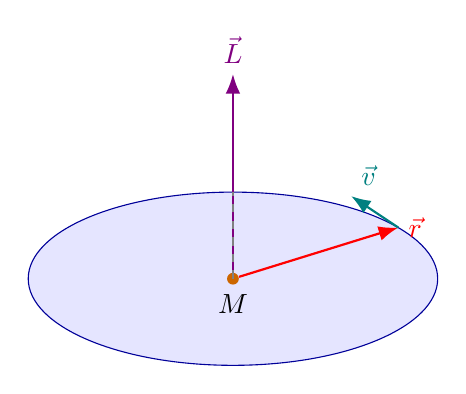
\begin{tikzpicture}[scale=1]
  \draw[fill=blue!10, draw=blue!60!black] (0,0) ellipse (2.6 and 1.1);
  \node[circle,fill=orange!80!black,inner sep=1.5pt,label=below:{$M$}] (F) at (0,0) {};
  \draw[-{Latex[length=2.5mm]}, thick, red] (F) -- (2.1,0.65) node[right] {$\vec r$};
  \draw[-{Latex[length=2.5mm]}, thick, teal] (2.1,0.65) -- (1.5,1.05) node[above right] {$\vec v$};
  \draw[-{Latex[length=2.5mm]}, thick, violet] (0,0) -- (0,2.6) node[above] {$\vec L$};
  \draw[dashed, gray] (0,0) -- (0,1.1);
\end{tikzpicture}
\end{center}
\begin{center}\textit{Figure 1: The orbital plane, pinned in place by the fixed direction of
$\vec L$. The planet's whole trajectory --- however complicated its shape --- lives entirely in
this one flat sheet.}\end{center}

\subsection{Setting Up the Motion: Polar Coordinates}

Since we now know the motion is confined to a plane, we only need two numbers to describe where
the planet is: a distance $r$ from the Sun, and an angle $\theta$ around it. This is a much more
natural choice than $x$ and $y$, because gravity itself only cares about $r$ --- so let's build our
description of motion out of coordinates gravity actually respects.

The subtlety with polar coordinates is that the "unit vectors" themselves rotate as the planet
moves --- $\hat r$ always points from the Sun to wherever the planet currently is, so as the planet
swings around, $\hat r$ swings with it. Working through the calculus of this rotation (a standard
but slightly fiddly exercise) gives velocity and acceleration as:
\[
\vec v = \dot r\hat r + r\dot\theta\hat\theta, \qquad
\vec a = (\ddot r - r\dot\theta^2)\hat r + (r\ddot\theta+2\dot r\dot\theta)\hat\theta.
\]
Don't worry about memorizing this derivation --- what matters is what happens next. Newton's
second law, $\vec F=m\vec a$, for a purely radial force, has no tangential ($\hat\theta$)
component at all. So the $\hat\theta$ part of $\vec a$ must be zero all by itself:
\[
r\ddot\theta + 2\dot r\dot\theta = 0 \quad\Longleftrightarrow\quad \frac{1}{r}\frac{d}{dt}(r^2\dot\theta) = 0
\quad\Longrightarrow\quad r^2\dot\theta = \text{constant}.
\]
Stop and notice something wonderful here: $mr^2\dot\theta$ is \emph{exactly} the magnitude of the
angular momentum $L$ we met a moment ago. We didn't need to invoke angular momentum conservation
as some separate fact handed down from above --- it fell right out of writing Newton's second law
in the coordinates that suit the problem. This is a recurring theme in physics: pick the right
coordinates, and the conservation laws practically write themselves.

\subsection{Kepler's Second Law: Equal Areas in Equal Times --- for Any Shape of Orbit}

Here's a lovely geometric fact hiding in that last equation. As the planet sweeps through a tiny
angle $d\theta$ at radius $r$, it traces out a thin, almost-triangular sliver of area,
\[
dA = \frac12 r^2\,d\theta
\]
(picture a very thin pizza slice --- its area is half the radius times the little arc it spans).
Divide by $dt$:
\[
\boxed{\frac{dA}{dt} = \frac12 r^2\dot\theta = \frac{L}{2m} = \text{constant}.}
\]
This is Kepler's Second Law, and notice we've proven it for \emph{any} orbit shape whatsoever ---
circular, elliptical, even the unbound parabolic and hyperbolic paths we'll meet shortly. It has
nothing specifically to do with orbits being ellipses; it's a direct, unavoidable consequence of
gravity being central, full stop.

The physical picture is worth internalizing: when a planet is close to the Sun (near perihelion),
it's moving \emph{fast}, sweeping through a wide angle very quickly. When it's far from the Sun
(near aphelion), it moves \emph{slowly}, crawling through only a small angle. But because the
close approach compensates with a wide angle and small radius, while the distant part compensates
with a narrow angle and large radius, the two effects trade off exactly, and equal areas get swept
in equal times, always. This is precisely why comets --- which have extremely eccentric orbits ---
spend the overwhelming majority of their orbital period crawling through the frigid outer solar
system, and only a brief, blazing moment whipping around the Sun at perihelion.

\begin{center}
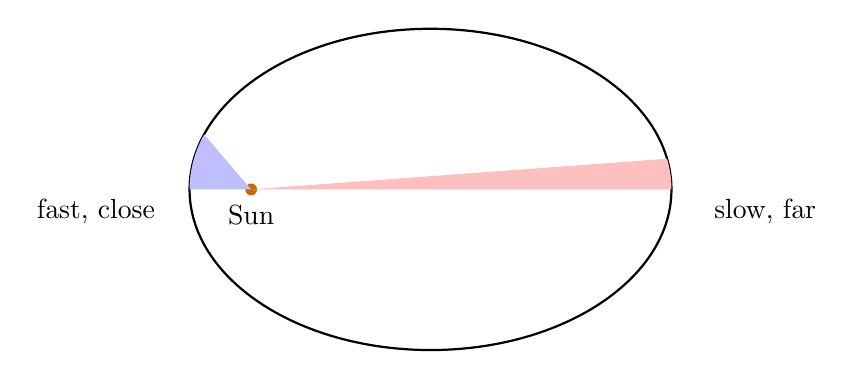
\begin{tikzpicture}[scale=0.85]
  \draw[thick] (0,0) ellipse (3.6 and 2.4);
  \coordinate (F) at (-2.68,0);
  \node[circle,fill=orange!80!black,inner sep=1.5pt,label=below:{Sun}] at (F) {};
  \fill[blue!25] (F) -- (-3.6,0) arc[start angle=180,end angle=160,x radius=3.6,y radius=2.4] -- cycle;
  \fill[red!25] (F) -- (3.6,0) arc[start angle=0,end angle=11,x radius=3.6,y radius=2.4] -- cycle;
  \node[below] at (-5,0) {fast, close};
  \node[below] at (5,0) {slow, far};
\end{tikzpicture}
\end{center}
\begin{center}\textit{Figure 2: The two shaded wedges have equal area, and were swept out in
equal time --- one very compressed in angle but close to the Sun, the other spread wide in angle
but very far away.}\end{center}

\subsection{Circular Orbits First: Kepler's Third Law, the Easy Way}

Before tackling the general, non-circular case, let's warm up with the simplest possible orbit: a
perfect circle. Here, the planet's speed never changes, and the only job gravity has is to
constantly redirect the planet's velocity so that it curves around instead of flying off in a
straight line. That redirecting force is exactly what we call centripetal force, and gravity
supplies it:
\[
\frac{GMm}{r^2} = m\omega^2 r, \qquad \omega=\frac{2\pi}{T}.
\]
Rearranging,
\[
\boxed{T^2 = \frac{4\pi^2}{GM}r^3.}
\]
Notice something curious already at this simple level: the bigger the orbit ($r$ larger), the
\emph{longer} the period, but not in a simple linear way --- it grows like $r^{3/2}$. Double the
orbital radius, and the period doesn't just double; it grows by a factor of $2\sqrt2\approx2.83$.
This is why Mercury, tucked in close to the Sun, zips around in just 88 days, while Neptune, way
out at the edge of the solar system, takes about 165 \emph{years} to complete a single orbit.

\subsection{Now the Real Question: What Shape is a Non-Circular Orbit?}

Circles are easy, but nature rarely gives us anything so tidy. Real orbits are ellipses, sometimes
quite eccentric ones. So the natural question is: given that gravity is a central, inverse-square
force, what \emph{shape} does the actual trajectory trace out? This is the derivation that let
Newton finally explain, from first principles, something Kepler had only guessed at from data:
that orbits are ellipses.

The trick is a clever change of variables. Instead of tracking $r$ as a function of time $t$
(which is messy, because both $r$ and $\theta$ are changing simultaneously and in a coupled way),
we're going to track $u \equiv 1/r$ as a function of the \emph{angle} $\theta$ instead. Why would
this help? Because we already know, from Kepler's second law, exactly how $\theta$ relates to
time: $\dot\theta = L/(mr^2) = Lu^2/m$. This lets us convert any time-derivative into a
$\theta$-derivative.

Working this through (differentiating $r=1/u$ with respect to $t$, using the chain rule and the
relation above, twice), the messy radial equation of motion
\[
m(\ddot r - r\dot\theta^2) = -\frac{GMm}{r^2}
\]
transforms, after some genuinely satisfying algebra, into
\[
\boxed{\frac{d^2u}{d\theta^2} + u = \frac{GMm^2}{L^2}.}
\]

Take a moment to appreciate how remarkable this equation is. If you've ever studied a mass on a
spring, or a pendulum swinging through small angles, you'll recognize this \emph{exact}
mathematical form --- it's the equation for simple harmonic motion, just with $\theta$ playing the
role that time usually plays! The messy, seemingly unrelated problem of planetary orbits has been
quietly transformed into a problem we already know how to solve, one that a student meets in their
very first weeks of studying oscillations.

The general solution to this "SHM in disguise" equation is a constant particular solution plus an
oscillating piece:
\[
u(\theta) = \frac{GMm^2}{L^2}\left[1+e\cos(\theta-\theta_0)\right].
\]
Choosing our angular reference point so that $\theta_0=0$ (measuring $\theta$ from the point of
closest approach) and flipping back to $r=1/u$:
\[
\boxed{r(\theta) = \frac{p}{1+e\cos\theta}}, \qquad p\equiv\frac1{k}=\frac{L^2}{GMm^2}.
\]

This is, precisely, the equation of a conic section in polar form, with one focus at the origin.
Depending on the value of $e$ (which is set by the orbit's energy and angular momentum, not chosen
freely), we get:
\begin{itemize}
\item $e=0$: a perfect circle.
\item $0<e<1$: an \textbf{ellipse}. This is Kepler's First Law, now not just observed but
\emph{derived}: bound orbits under gravity must be ellipses (or the special case of a circle).
\item $e=1$: a parabola --- an orbit that is only just barely unbound, arriving at infinity with
exactly zero leftover speed.
\item $e>1$: a hyperbola --- a genuinely unbound trajectory, like a comet passing through once and
never returning, or a spacecraft on a flyby.
\end{itemize}

\begin{center}
\begin{tikzpicture}[scale=0.85]
  \draw[thick] (0,0) ellipse (3.6 and 2.4);
  \coordinate (F1) at (-2.683,0);
  \node[circle,fill=orange!80!black,inner sep=1.8pt,label=above:{$F_1$}] at (F1) {};
  \draw[dashed] (-3.6,0) -- (3.6,0);
  \node[below left] at (-3.6,0) {$r_p=a(1-e)$};
  \node[below right] at (3.6,0) {$r_a=a(1+e)$};
  \draw[-{Latex[length=2mm]}] (0,0) -- (3.6,0) node[midway, above] {$a$};
\end{tikzpicture}
\end{center}
\begin{center}\textit{Figure 3: The Sun sits at a focus of the ellipse $F_1$ --- not at the geometric
center, a detail that surprises many people the first time they think carefully about it.}\end{center}

\subsection{A Different Lens: Thinking in Terms of Energy}

There's a second, equally illuminating way to understand the shape of an orbit, and it's worth
learning both because different problems will suit different approaches. Instead of tracking the
orbit's geometric shape directly, let's track its energy.

The gravitational potential energy comes from asking: how much work does it take to move a mass
from radius $r$ out to infinity, fighting against gravity the whole way? Integrating the force:
\[
U(\infty)-U(r) = -\int_r^\infty\left(-\frac{GMm}{r'^2}\right)dr' = -\frac{GMm}{r}.
\]
With the natural convention $U(\infty)=0$ (two masses infinitely far apart don't interact, so
there's no stored energy between them), we get the familiar
\[
\boxed{U(r) = -\frac{GMm}{r}.}
\]
The negative sign here is worth pausing on: it tells us that a bound system (planet orbiting
Sun) has \emph{less} total energy than two masses sitting infinitely far apart at rest. That makes
intuitive sense --- you'd have to \emph{add} energy to the system to pull the planet away to
infinity, so being bound must correspond to an energy deficit relative to being unbound.

Now, using $v^2=\dot r^2+r^2\dot\theta^2$ and the fact that $r^2\dot\theta=L/m$ is fixed, the total
mechanical energy becomes
\[
E = \frac12m\dot r^2 + \underbrace{\frac{L^2}{2mr^2} - \frac{GMm}{r}}_{\displaystyle V_{\text{eff}}(r)}.
\]
We've bundled the angular-momentum piece together with the potential energy into something called
the \textbf{effective potential}, $V_{\text{eff}}(r)$. Why is this useful? Because now the problem
\emph{looks} exactly like a one-dimensional particle moving under some potential $V_{\text{eff}}$
--- as if the planet were a marble rolling around in a valley whose shape is given by this curve,
with $r$ playing the role of horizontal position. The genuinely two-dimensional orbit problem has
been squashed down into a much more familiar-looking one-dimensional problem.

\begin{center}
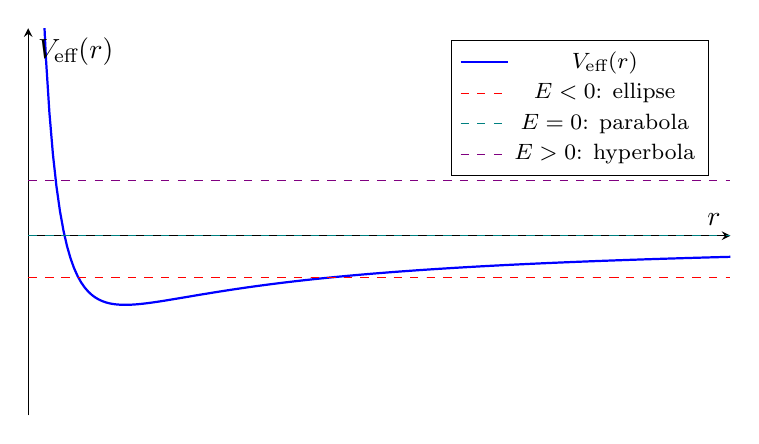
\begin{tikzpicture}
\begin{axis}[width=10.5cm, height=6.5cm, xlabel={$r$}, ylabel={$V_{\text{eff}}(r)$},
  xmin=0.2, xmax=6, ymin=-1.3, ymax=1.5, axis lines=middle, ytick=\empty, xtick=\empty,
  domain=0.2:6, samples=200, legend pos=north east, legend style={font=\footnotesize}]
  \addplot[thick, blue] {1/(2*x^2) - 1/x};
  \addlegendentry{$V_{\text{eff}}(r)$}
  \addplot[dashed, red] {-0.3}; \addlegendentry{$E<0$: ellipse}
  \addplot[dashed, teal] {0}; \addlegendentry{$E=0$: parabola}
  \addplot[dashed, violet] {0.4}; \addlegendentry{$E>0$: hyperbola}
\end{axis}
\end{tikzpicture}
\end{center}
\begin{center}\textit{Figure 4: The effective-potential ``valley.'' Wherever a horizontal energy
line crosses the curve marks a turning point of the real orbit --- the perihelion and aphelion
distances. Notice the curve blows up to $+\infty$ as $r\to0$: this is the angular-momentum barrier
(sometimes called the centrifugal barrier), and it's the reason a planet with any angular momentum
at all can never actually crash straight into the Sun --- it always gets "turned around" first, no
matter how close it gets.}\end{center}

Think about what this diagram is really telling you. If the total energy $E$ is negative, the
"marble" doesn't have enough energy to climb out of the valley on the right side (toward
$r\to\infty$, where $V_{\text{eff}}\to0$), so it's trapped, oscillating back and forth between two
turning points forever --- that's a bound, elliptical orbit. If $E$ is exactly zero, the marble
\emph{just barely} makes it out to $r=\infty$ with no speed left over --- a parabola. If $E$ is
positive, the marble sails out to infinity with speed to spare --- a hyperbola. This single picture
contains the entire classification of orbit types, and you didn't need to solve any differential
equation to get it; you just needed to know the shape of one curve.

\subsection{Back to Kepler's Third Law: Now for Any Ellipse}

We derived Kepler's Third Law earlier for the special case of a circle. Let's now get the fully
general result for an ellipse of any eccentricity, using the equal-areas result from earlier as
our tool.

Over one full orbital period $T$, the radius vector must sweep out the \emph{entire} area of the
ellipse, which is $\pi ab$ (a standard geometric fact: an ellipse with semi-axes $a$ and $b$ has
area $\pi ab$, generalizing the familiar circle formula $\pi r^2$). Since the rate of area-sweeping
is constant at $L/2m$,
\[
\pi ab = \frac{L}{2m}T \quad\Longrightarrow\quad T = \frac{2m\pi ab}{L}.
\]
Now we need to relate $L$ back to the orbit's shape. Comparing $p=b^2/a$ (a standard geometric
relation for ellipses) to our earlier expression $p=L^2/(GMm^2)$, we can solve for $L$ in terms of
the shape parameters, and substituting back in gives, after the dust settles,
\[
\boxed{T^2 = \frac{4\pi^2}{GM}a^3.}
\]
This is, remarkably, the \emph{exact same formula} we found for a circular orbit, just with the
circle's radius $r$ replaced by the ellipse's semi-major axis $a$. The period doesn't care at all
about the eccentricity --- two orbits with wildly different shapes (one nearly circular, one a
long thin sliver) but the same semi-major axis will complete their journeys in exactly the same
amount of time. If that feels surprising, it should --- it's one of the genuinely elegant surprises
buried inside Newton's law.

\subsection{The Vis-Viva Equation: Speed Anywhere on the Orbit}

Here's a practical question a lot of orbital-mechanics problems boil down to: given that a
spacecraft (or planet, or comet) is at some particular distance $r$ from the central body, how
fast is it moving \emph{right now}?

We could, in principle, always go back to conserving energy and angular momentum separately every
single time, but there's a shortcut worth having in your toolkit. It turns out (and can be checked
directly by evaluating the energy at the perihelion point, where all the algebra simplifies nicely)
that the total energy of \emph{any} bound Keplerian orbit depends \emph{only} on its semi-major
axis, not on its eccentricity:
\[
E = -\frac{GMm}{2a}.
\]
Setting this equal to our general expression for energy, $E=\frac12mv^2-GMm/r$, and solving for
$v^2$:
\[
\boxed{v^2 = GM\left(\frac2r-\frac1a\right).}
\]
This little equation is a real workhorse. Notice what it's telling you: speed depends on where you
currently are ($r$) relative to the overall size of the orbit ($a$). Near perihelion, where $r$ is
smallest, the $2/r$ term dominates and speed is largest. Near aphelion, where $r$ is largest, speed
drops. This matches the intuition we already built from Kepler's Second Law --- of course the
planet moves fastest when closest and slowest when farthest, but now we have the precise
quantitative relationship, not just the qualitative trend.

\subsection{Escape Velocity, and What "Energy $\geq0$" Really Means}

What if a planet, or a rocket, has \emph{so much} energy that it never comes back at all? We
already saw a hint of this in the effective potential picture: it happens exactly when $E\geq0$.
Let's find the critical launch speed for this to happen from some radius $R$.

The threshold case is $E=0$ exactly --- just barely escaping, arriving at infinity with zero speed
left over (like throwing a ball up with just enough speed that it "stops" infinitely far away,
never quite falling back, but never having extra speed to spare either). Setting
$E=\frac12mv_{\text{esc}}^2-GMm/R=0$:
\[
\boxed{v_{\text{esc}} = \sqrt{\frac{2GM}{R}}.}
\]
Compare this to the speed needed for a circular orbit at the same radius,
$v_{\text{circ}}=\sqrt{GM/R}$ (which you can get directly from Section 2.4's centripetal-force
balance). The ratio is a clean, memorable number:
\[
v_{\text{esc}} = \sqrt2\ v_{\text{circ}}.
\]
This holds at \emph{any} radius, for \emph{any} central mass --- a useful fact to keep in your back
pocket, since it lets you get escape velocity for free whenever you already know the circular
orbital speed, and vice versa.

Putting it all together, the sign of the total energy is really a complete classification scheme
for the whole \emph{type} of trajectory a body can have:

\begin{center}
\begin{tabular}{ccc}
$E<0$ & $E=0$ & $E>0$ \\
ellipse, permanently bound & parabola, marginally escapes & hyperbola, escapes with speed to spare
\end{tabular}
\end{center}

\section{Roche Limit}

Here's a question with a slightly unsettling answer: can a moon get \emph{too close} to its
planet and simply be torn apart? The answer is yes, and understanding why requires appreciating
that gravity isn't uniform --- it's slightly stronger on the near side of an object than on the far
side, and that difference, small as it usually is, can become catastrophic at close range.

Picture a satellite orbiting close to a planet. The side of the satellite facing the planet is,
by definition, a little bit closer to the planet's center than the satellite's own center is; the
far side is a little farther. Since gravity falls off with distance, the near side feels a
noticeably stronger pull than the center does, and the far side feels a noticeably weaker pull.
The result is that the satellite is being \emph{stretched} --- pulled apart along the line joining
it to the planet, like a piece of taffy being pulled from both ends, even though nothing is
grabbing the far side at all; it's simply being left behind relative to how hard the near side is
being tugged.

Let's put a number on this stretching. If the satellite has radius $r_s$ and its center is at
distance $d$ from the planet (mass $M$), the near side sits at distance $(d-r_s)$. Expanding to
leading order in the (presumably small) ratio $r_s/d$:
\[
g_{\text{near}} = \frac{GM}{(d-r_s)^2} \approx \frac{GM}{d^2}\left(1+\frac{2r_s}{d}\right).
\]
The excess pull, over and above what the satellite's center feels, is the tidal acceleration:
\[
\boxed{a_{\text{tidal}} \approx \frac{2GM\,r_s}{d^3}.}
\]
Notice this falls off as $1/d^3$, faster than ordinary gravity's $1/d^2$ --- which is exactly why
tidal effects, while often negligible far away, can become dominant and even destructive at close
range. It's a difference-of-forces effect, and differences shrink faster than the forces
themselves as you back away.

Now, what's holding the satellite together against this stretching in the first place? Its own
self-gravity, pulling surface material back toward its own center:
\[
a_{\text{self}} = \frac{Gm_s}{r_s^2}.
\]
The satellite survives as long as self-gravity wins. It comes apart exactly when the two are equal
--- this defines a critical distance, the Roche limit $d_R$:
\[
\frac{2GM\,r_s}{d_R^3} = \frac{Gm_s}{r_s^2} \quad\Longrightarrow\quad d_R^3 = \frac{2M\,r_s^3}{m_s}.
\]
This still has the satellite's own size and mass tangled up in it, which isn't the most convenient
form. Let's rewrite everything in terms of \emph{mean densities} instead --- $\rho_M$ for the
planet, $\rho_s$ for the satellite --- using $M=\frac43\pi R^3\rho_M$ and $m_s=\frac43\pi
r_s^3\rho_s$. Substituting, the factors of $r_s^3$ cancel completely, leaving a wonderfully clean
result:
\[
\boxed{d_R = R\left(\frac{2\rho_M}{\rho_s}\right)^{1/3}.}
\]
The satellite's actual size dropped out entirely! All that matters is the \emph{contrast} in
density between planet and satellite, measured in units of the planet's own radius. A dense, rocky
moon can survive much closer to its planet than a loosely-packed, icy or rubble-pile object could
--- which is exactly the physical reason Saturn's icy rings sit where they do: they're made of
material that simply couldn't hold itself together as a single moon any closer in.

\begin{center}
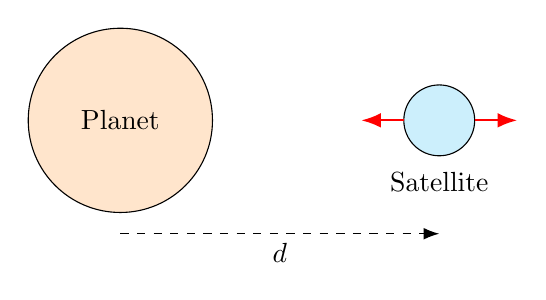
\begin{tikzpicture}[scale=0.9]
  \draw[fill=orange!20] (0,0) circle (1.3); \node at (0,0) {Planet};
  \draw[fill=cyan!20] (4.5,0) circle (0.5); \node[below] at (4.5,-0.6) {Satellite};
  \draw[-{Latex[length=2.5mm]}, thick, red] (4.0,0) -- (3.4,0);
  \draw[-{Latex[length=2.5mm]}, thick, red] (5.0,0) -- (5.6,0);
  \draw[-{Latex[length=2mm]}, dashed] (0,-1.6) -- (4.5,-1.6) node[midway, below] {$d$};
\end{tikzpicture}
\end{center}
\begin{center}\textit{Figure 5: The satellite is stretched along the line joining it to the
planet --- pulled toward the planet on the near side, and effectively left behind on the far side.
Below $d_R$, this stretching overwhelms the satellite's self-gravity.}\end{center}

\section{Barycentre}

So far we've been quietly assuming that one body (the "Sun," or the "planet") just sits still
while the other orbits around it. That's a fine approximation when one mass hugely outweighs the
other, but it's not quite the truth, and it's worth being honest about what's really going on ---
especially because binary star systems (two comparable-mass stars) show the effect very clearly.

The truth is: \emph{both} bodies orbit. They orbit a shared point called the barycentre, or center
of mass, defined the same way you'd define a center of mass for any system:
\[
\vec R_{\text{cm}} = \frac{M_1\vec r_1+M_2\vec r_2}{M_1+M_2}.
\]
If we choose to view the system from a reference frame where this point sits at the origin (a
completely legitimate and often very convenient choice), then at every single instant,
\[
M_1\vec r_1 = -M_2\vec r_2.
\]
Read this carefully: it says the two position vectors, measured from the barycentre, always point
in exactly opposite directions, and their magnitudes are in inverse proportion to the masses. Think
of two children of very different weights on a seesaw --- for the seesaw to balance, the heavier
child has to sit much closer to the pivot than the lighter one. It's exactly the same idea here,
except now the "seesaw" is spinning: both stars trace out their own ellipses, similar in shape,
but scaled so the heavier star's ellipse is proportionally smaller and hugs closer to the shared
center.

This isn't just a geometric curiosity --- it's directly useful for astronomers, because we can
often measure the individual speeds of two stars in a binary system (via how their light is
Doppler-shifted as they move toward and away from us), even when we can't easily measure their
individual distances. Since both stars share the exact same orbital period (they have to, since
they must remain collinear with the barycentre at all times), and since $r_1/r_2=M_2/M_1$ always,
it follows immediately that
\[
\frac{v_1}{v_2} = \frac{r_1}{r_2} = \frac{M_2}{M_1}.
\]
Just from a ratio of observed speeds, you get the mass ratio of two stars you may never even be
able to resolve as separate points of light. This is one of the quiet triumphs of celestial
mechanics: turning something as simple as "which star's light wobbles more" into a hard number for
how much more massive one star is than the other.

\begin{center}
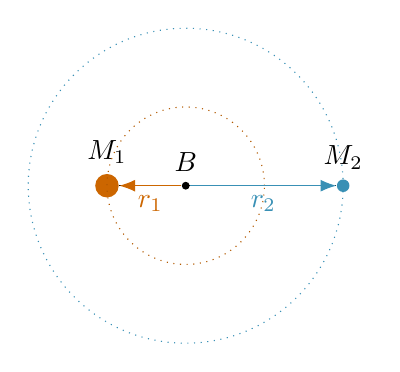
\begin{tikzpicture}[scale=1]
  \node[circle,fill=orange!80!black,inner sep=3pt,label=above:{$M_1$}] (M1) at (-1,0) {};
  \node[circle,fill=cyan!70!black,inner sep=1.6pt,label=above:{$M_2$}] (M2) at (2,0) {};
  \node[circle,fill=black,inner sep=1pt,label=above:{$B$}] (COM) at (0,0) {};
  \draw[dashed] (M1) -- (M2);
  \draw[dotted, orange!70!black] (0,0) circle (1);
  \draw[dotted, cyan!70!black] (0,0) circle (2);
  \draw[-{Latex[length=2mm]}, orange!80!black] (COM) -- (M1) node[midway, below] {$r_1$};
  \draw[-{Latex[length=2mm]}, cyan!70!black] (COM) -- (M2) node[midway, below] {$r_2$};
\end{tikzpicture}
\end{center}
\begin{center}\textit{Figure 6: The heavier star ($M_1$) stays closer to the shared barycentre $B$;
the lighter star ($M_2$) swings around on a wider circuit. Both always remain on exactly opposite
sides of the barycentre.}\end{center}

\section{Two-Body Problem}

There's something a little unsatisfying about the previous section. We described \emph{where}
each star sits relative to the barycentre, but we never actually justified treating the barycentre
as if it doesn't move, or explained precisely why we're allowed to reuse all of the single-body
machinery from Section 2 (Kepler's laws, vis-viva, and so on) for a system where \emph{both}
bodies are moving. Let's fix that properly.

\subsection*{Splitting the Motion in Two}

Define the relative separation vector $\vec r=\vec r_1-\vec r_2$ (how far apart the two bodies are,
and in what direction), alongside the barycentre position $\vec R_{\text{cm}}$ we already met.
Using the relations $\vec r_1=\vec R_{\text{cm}}+\frac{M_2}{M_1+M_2}\vec r$ and
$\vec r_2=\vec R_{\text{cm}}-\frac{M_1}{M_1+M_2}\vec r$, let's compute the \emph{total} kinetic
energy of the system and see what happens:
\[
KE = \frac12M_1|\dot{\vec r}_1|^2+\frac12M_2|\dot{\vec r}_2|^2
= \frac12(M_1+M_2)|\dot{\vec R}_{\text{cm}}|^2 + \frac12\mu|\dot{\vec r}|^2,
\]
where all the cross-terms between $\dot{\vec R}_{\text{cm}}$ and $\dot{\vec r}$ cancel out neatly
(a small algebraic miracle worth checking for yourself once), and a new quantity has appeared:
\[
\boxed{\mu \equiv \frac{M_1M_2}{M_1+M_2}}, \qquad \text{the \textbf{reduced mass}}.
\]
This is a genuinely beautiful result. It says that the total kinetic energy of \emph{two} moving
bodies splits, with no leftover cross-terms, into exactly two independent pieces: the kinetic
energy of the total mass $M_1+M_2$ moving as if concentrated at the barycentre, plus the kinetic
energy of a single \emph{fictitious} particle of mass $\mu$, moving with the relative velocity
$\dot{\vec r}$.

\subsection*{Why This Matters}

Because gravity conserves total momentum (Newton's third law guarantees the two gravitational
forces on the two bodies are equal and opposite), the barycentre moves in a straight line at
constant velocity, forever, completely unaffected by whatever complicated dance the two bodies do
around it. All the \emph{interesting} physics --- the actual shape of the orbit, how fast the
separation changes, the period --- lives entirely in the second piece: the relative motion of our
fictitious particle of mass $\mu$.

And how does this fictitious particle move? Applying Newton's second law to the relative
coordinate directly:
\[
\mu\ddot{\vec r} = -\frac{GM_1M_2}{r^2}\hat r \quad\Longrightarrow\quad
\ddot{\vec r} = -\frac{G(M_1+M_2)}{r^2}\hat r.
\]
Notice that $\mu$ actually cancels out of the equation of motion entirely (it appears on both
sides, since the gravitational force itself is proportional to $M_1M_2 = \mu(M_1+M_2)$) --- so this
equation is \emph{exactly} the single-body equation of motion we started with all the way back in
Section 2, just with the single mass $M$ replaced by the total mass $M_1+M_2$.

This is the real justification for something we may have been doing on faith so far: every result
we derived for a planet orbiting a fixed Sun --- Kepler's three laws, the vis-viva equation, the
whole effective-potential picture --- transfers over immediately and exactly to a two-body system,
provided you make one substitution: replace the single central mass $M$ with the total mass
$M_1+M_2$, and understand that $a$, $r$, and so on now refer to the \emph{relative} separation
between the two bodies, not the distance of one from some fixed point.

\begin{aside}{An Aside: Why Bother With $\mu$ At All?}
You might wonder why we introduced this "reduced mass" business at all, since it seems to cancel
out of the final equation of motion anyway. The honest answer is: it doesn't cancel out of
\emph{everything} --- it's essential for correctly computing the system's total energy and angular
momentum (both of which genuinely depend on $\mu$, not on $M_1+M_2$), and it's the rigorous reason
we're allowed to treat "two bodies orbiting each other" as equivalent to "one body orbiting a fixed
point" in the first place. Physicists reach for this trick constantly, well beyond gravity ---
it shows up identically in the quantum mechanics of a hydrogen atom, where the electron and proton
technically both orbit their shared center of mass too.
\end{aside}

\section{Lagrange Points}

Here's a genuinely delightful question to end on: are there any special places, near a two-body
system like the Earth and the Sun, where a third, much smaller object (a spacecraft, an asteroid)
could sit and simply \emph{stay put}, neither drifting toward one body nor the other, held in
place by the combined tug-of-war of both?

At first, this sounds like it shouldn't be possible except right at the barycentre, in a completely
static, non-orbiting situation. But that's not actually the right way to think about it, because
our small object doesn't need to be motionless in any absolute sense --- it just needs to keep pace
with the rotation of the whole system, orbiting the barycentre with exactly the same period as the
two main bodies do. If it manages that, then from the point of view of an observer standing on
one of the two main bodies (co-rotating with them), the small object would appear perfectly
stationary, even though, from far away, everyone involved is actually sweeping around in a circle
together.

This is the trick: switch to a \textbf{rotating reference frame}, one that spins right along with
$M_1$ and $M_2$ at their shared orbital angular velocity $\omega=\sqrt{G(M_1+M_2)/a^3}$ (Kepler's
Third Law again, doing double duty). In this frame, $M_1$ and $M_2$ both look perfectly still,
frozen in place on the $x$-axis. But because we're in a \emph{rotating} frame, we have to add in a
fictitious force to account for the rotation --- the same centrifugal effect you feel pressed
outward against a car door as it turns a sharp corner.

Combining real gravity from both bodies with this fictitious centrifugal effect, we can define an
effective potential for the rotating frame:
\[
\Phi_{\text{eff}}(x,y) = -\frac{GM_1}{r_1}-\frac{GM_2}{r_2}-\frac12\omega^2(x^2+y^2),
\]
where $r_1$ and $r_2$ are the distances from our small test object to $M_1$ and $M_2$
respectively. A \textbf{Lagrange point} is simply a place where this potential is "flat" ---
$\nabla\Phi_{\text{eff}}=0$ --- meaning a test mass placed exactly there, at rest in this rotating
frame, feels no net push in any direction, and so just sits there.

\subsection*{The Three Points on the Line: $L_1$, $L_2$, $L_3$}

The easiest points to find are the ones lying directly on the line joining $M_1$ and $M_2$
(extended in both directions), since the geometry there is one-dimensional. Let's specialize to the
very common and intuitive case $M_2\ll M_1$ --- think of the Sun and the Earth. Somewhere between
the two bodies, gravity from the Sun (pulling one way) and gravity from Earth (pulling the other
way), together with the centrifugal effect, must all balance. Writing this balance for a small
displacement $r$ of this point from Earth, toward the Sun:
\[
\frac{GM_1}{(a-r)^2} - \frac{GM_2}{r^2} = \omega^2(a-r).
\]
Expanding the left side to leading order in the small quantity $r/a$, and using
$\omega^2\approx GM_1/a^3$ (an excellent approximation here since $M_2\ll M_1$), the large $GM_1$
terms on both sides very nearly cancel each other, leaving behind only the small corrections. What
survives, after simplifying, is a beautifully compact result:
\[
\boxed{r_{L_1} \approx a\left(\frac{M_2}{3M_1}\right)^{1/3}.}
\]
This is the point, between the Earth and the Sun, where the Sun's stronger pull is just barely
balanced by the combination of Earth's much weaker (but much closer!) pull and the centrifugal
effect. It's precisely why spacecraft like SOHO, which stares continuously at the Sun, are parked
at $L_1$ --- close enough to Earth for easy communication, but positioned so they orbit the Sun in
lockstep with Earth rather than drifting away.

By an almost identical calculation on the \emph{far} side of Earth (away from the Sun), we find a
second point, $L_2$, at essentially the same distance:
\[
\boxed{r_{L_2} \approx a\left(\frac{M_2}{3M_1}\right)^{1/3}.}
\]
This is where missions like the James Webb Space Telescope are stationed --- shielded from the
Sun by Earth, while still keeping pace with Earth's orbit rather than falling behind.

There's a third collinear point, $L_3$, tucked away on the far side of the Sun, almost exactly
opposite Earth. Because it's so far from Earth, Earth's gravity barely perturbs the Sun's field
there at all, and the correction to a pure Sun-only orbit is correspondingly tiny:
\[
r_{L_3} \approx a\left(1+\frac{5M_2}{12M_1}\right) \text{ (measured from the Sun)}.
\]

\subsection*{The Two Off-Axis Points: $L_4$ and $L_5$}

The remaining two Lagrange points are, in some ways, the most surprising and elegant of the five.
They don't sit on the line between $M_1$ and $M_2$ at all --- instead, picture forming an
\emph{equilateral triangle}, using the $M_1$--$M_2$ separation $a$ as one side, with the third
vertex either leading or trailing $M_2$ in its orbit. Remarkably, both of these triangular points
are equilibria, for \emph{any} mass ratio at all --- not just special cases.

Here's the intuition for why. At either triangular point, gravity from $M_1$ pulls with strength
$GM_1m/a^2$ along one side of the triangle, and gravity from $M_2$ pulls with strength
$GM_2m/a^2$ along the other side, with exactly a $60^\circ$ angle between these two directions
(fixed purely by the equilateral geometry, regardless of the actual masses involved). If you add
these two force vectors together --- treating it as a straightforward exercise in vector addition
--- something rather magical happens: the resultant force points \emph{exactly} toward the
barycentre of the $M_1$-$M_2$ system, and its magnitude is \emph{exactly} the right amount needed
to keep the test mass moving in a circle of that particular radius, at that particular angular
velocity $\omega$, around that particular barycentre. Gravity, all on its own, conspires to supply
precisely the centripetal force needed --- no extra fine-tuning of the mass ratio required. It's a
genuine gift from the geometry of the equilateral triangle, combined with how a barycentre divides
the line between two masses.

\begin{center}
\begin{tikzpicture}[scale=1.0]
  \node[circle,fill=orange!80!black,inner sep=3.5pt,label=above:{$M_1$}] (M1) at (-2,0) {};
  \node[circle,fill=cyan!70!black,inner sep=2pt,label=above:{$M_2$}] (M2) at (2,0) {};
  \node[circle,fill=black,inner sep=1pt,label=below:{$B$}] (COM) at (-1.2,0) {};
  \draw[dashed] (-4.5,0) -- (5,0);
  \node[circle,fill=red!70!black,inner sep=1.5pt,label=above:{$L_1$}] at (0.8,0) {};
  \node[circle,fill=red!70!black,inner sep=1.5pt,label=above:{$L_2$}] at (3.1,0) {};
  \node[circle,fill=red!70!black,inner sep=1.5pt,label=above:{$L_3$}] at (-4.1,0) {};
  \node[circle,fill=red!70!black,inner sep=1.5pt,label=above:{$L_4$}] at (0,3.46) {};
  \node[circle,fill=red!70!black,inner sep=1.5pt,label=below:{$L_5$}] at (0,-3.46) {};
  \draw[gray, thin] (M1) -- (0,3.46) -- (M2) -- cycle;
  \draw[gray, thin] (M1) -- (0,-3.46) -- (M2) -- cycle;
\end{tikzpicture}
\end{center}
\begin{center}\textit{Figure 7: The five Lagrange points. $L_1$, $L_2$, $L_3$ lie strung out
along the line joining $M_1$ and $M_2$; $L_4$ and $L_5$ sit at the apex of equilateral triangles
built on the $M_1$-$M_2$ separation (drawn here with a comparable-mass ratio for visual clarity
--- for $M_2\ll M_1$, the three collinear points crowd close in near $M_2$ and far out beyond
$M_1$, while $L_4$/$L_5$ remain roughly the same distance from the Sun as $M_2$ itself).}\end{center}

\subsection*{A Note on Stability}

It's worth knowing, even without working through the full stability analysis (which involves
looking at the curvature of $\Phi_{\text{eff}}$ in all directions around each point, not just
whether the gradient vanishes there), that these five points are not all equally "comfortable"
places to sit. $L_1$, $L_2$, and $L_3$ are always \textbf{unstable} --- nudge an object slightly
off one of these points, and it will drift away rather than being pulled back, rather like trying
to balance a marble exactly on top of a hill. Spacecraft parked there need occasional small
thruster corrections to stay put.

$L_4$ and $L_5$, by contrast, \emph{can} be stable --- but only if the mass ratio $M_1/M_2$
exceeds roughly $24.96$. Happily, this condition is comfortably satisfied for the Sun-Earth,
Sun-Jupiter, and Earth-Moon systems, which is exactly why we observe swarms of Trojan asteroids
happily orbiting near Jupiter's $L_4$ and $L_5$ points, having sat there stably for billions of
years without any need for active correction.

\section{Summary Sheet}

\begin{center}
\renewcommand{\arraystretch}{1.6}
\begin{tabular}{|l|l|}
\hline
\textbf{Topic} & \textbf{Result} \\
\hline
Newton's law & $F = GMm/r^2$, always attractive \\
Kepler II (any orbit) & $dA/dt = L/2m = $ const. \\
Kepler III (circular \& elliptical) & $T^2 = 4\pi^2 a^3/GM$ \\
Vis-viva & $v^2 = GM(2/r - 1/a)$ \\
Escape velocity & $v_{\text{esc}} = \sqrt{2GM/R} = \sqrt2\,v_{\text{circ}}$ \\
Roche limit & $d_R = R(2\rho_M/\rho_s)^{1/3}$ \\
Barycentre & $M_1 r_1 = M_2 r_2$; \ $v_1/v_2 = M_2/M_1$ \\
Two-body reduction & $\mu = M_1M_2/(M_1+M_2)$; relative orbit uses $M_1+M_2$ \\
Lagrange $L_1, L_2$ & $r \approx a(M_2/3M_1)^{1/3}$ from $M_2$ \\
Lagrange $L_4, L_5$ & equilateral triangle with $M_1, M_2$; stable if $M_1/M_2 \gtrsim 24.96$ \\
\hline
\end{tabular}
\end{center}

\section{Further Reading}
I mainly wrote this handout to build intuition for celestial mechanics, rather than problem solving capability. For Olympiad-level problem solving and mathematical rigor, use these!

\begin{itemize}
    \item \href{https://aoguide.app}{\textbf{Astronomy Olympiad Guide}}: A highly optimized learning platform built by former contestants (including IOAA Gold Medalists) to bridge the massive gap between dry university textbooks and competitive problem sheets. It breaks the entire syllabus down into clean, manageable core study tracks.
    \item \href{https://aoguide.app}{\textbf{aoXiv Archive}}: The definitive comprehensive global repository of astronomy and astrophysics olympiad papers. It hosts an organized, searchable collection of official problems, solutions, and grading schemes from international (IOAA), regional, and national competitions (such as USAAAO, NSEA, and BAAO).
    \item \href{https://drive.google.com/file/d/1RM__5pGAsbDip_k_N2zqHnHW_xXBau_G/view}{\textbf{Orbital Mechanics Handout} by ongzz}: A legendary, mathematically comprehensive deep-dive handout that walks through advanced orbital transformations, coordinate system dynamics, and elite-tier mechanics proofs with spectacular precision.
    \item \href{https://drive.google.com/file/d/1V12rbls_OdmsxS4HSG2sudghqPZ54Wfz/view}{\textbf{An Introduction to Modern Astrophysics} by Carroll \& Ostlie (The "BOB")}: The absolute baseline bible for undergraduate astrophysics. Chapters 2 and 10 provide the gold-standard reference for rigorous orbital proofs and binary systems.
    \item \href{https://drive.google.com/file/d/1gFn2rYAE5QMrge7B0cz1x4K12mr2Ca1s/view}{\textbf{Problems and Solutions in Astronomy and Astrophysics} by Dr. Aniket Sule}: A premium collection of past international competition problems complete with fully unrolled solution keys categorized by subject area.
    \item \href{https://drive.google.com/file/d/1jAAtkF0YCrT3Fm9B4I2kxez393olF_iy/view}{\textbf{Fundamental Astronomy} by Hannu Karttunen et al.}: Excellent for connecting planetary geometry directly to celestial coordinate frameworks and spherical trigonometry expansions.
\end{itemize}

\end{document}